

\chapter{Chapter heading}
\indent Write the body of the thesis. Include as many chapters as needed.


\section{Sections in chapter}

Logically divide the content of the chapter into sections and subsections. 


\subsection{An example subsection}

Within a subsection, content division may again be included as shown below.

\subsubsection{Examples of equations}

\indent  A few examples of various types of equations are shown in Eq.~\ref{eq:A(z)}, to Eq.~\ref{eq:vs1}.

\begin{equation}
  	A(\emph{z})= \frac{1-B(\emph{z})}{1-B(\frac{z}{\gamma})}
  	\label{eq:A(z)}
\end{equation}

\begin{equation}
	A(\frac{z}{\gamma})=\sum\limits_{i=1}^M \gamma^{i} x_{i}z^{-i}, 0 < \gamma < 1
  	\label{eq:A(z/gamma)}
\end{equation}

\begin{equation}
  	a_{n}^{'}=
	\begin{cases}

	a_{n}b_{n},& 0\le{n}\le{N-1}\\
   	 0,              & \text{otherwise}
	\end{cases}
  \label{eq:andash}
  \end{equation}


\begin{equation}
  a_{n}= \alpha - \beta \cos \frac{2 \pi n}{N-1}
  \label{eq:an}
  \end{equation}
where \(\alpha = 0.54\) and \(\beta = 1-\alpha = 0.46\).


\begin{equation}
\frac{\delta C}{\delta a_{k}} = 2E[(s[n] + \sum\limits_{k=1}^M (a_{k}s_{n-k}))b_{n-i}] = 0
  \label{eq:dC}
  \end{equation}

\begin{equation}
A=\lVert \mathbf{x}(n) - \eta_{k}b_{i}\mathbf{C}y_j \rVert 
  \label{eq:Alvert}
  \end{equation}

\begin{equation}
  a_{1}= b[T^{(1)}]
  \label{eq:vs1}
  \end{equation}

\subsubsection{Examples of figures}

\indent Figures may be included as in Fig.~\ref{fig:CELPdecth}. To increase or decrease the size of the figures, adjust the `scale' parameter in the code. 
\begin{figure}[h]
      \begin{center}
                 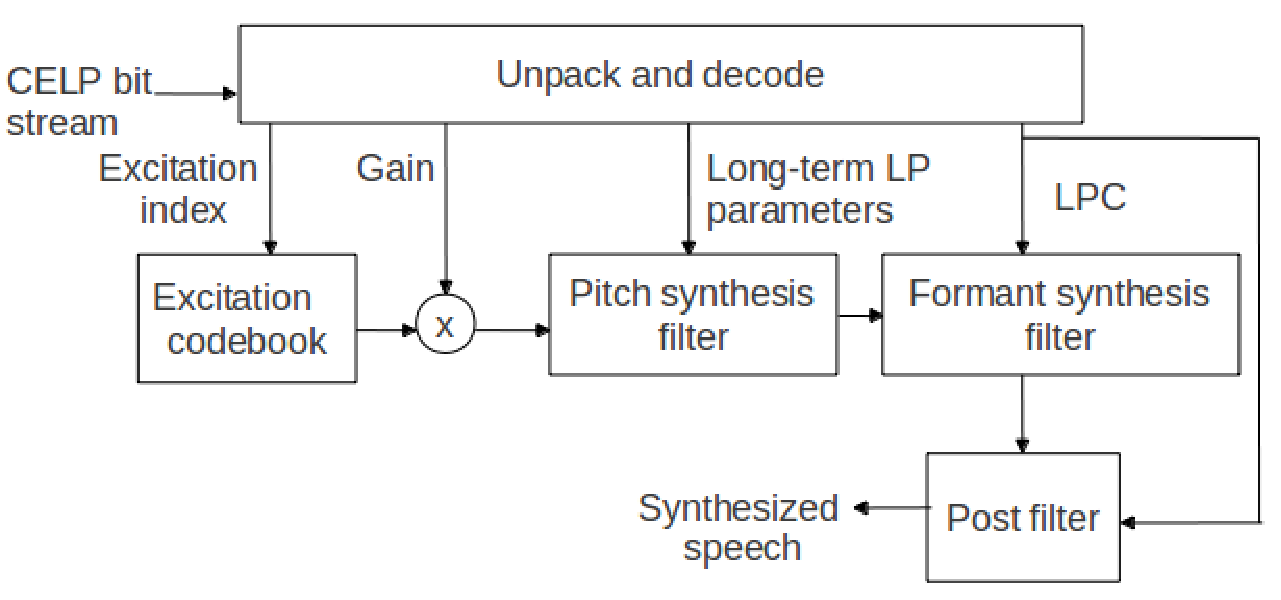
\includegraphics[scale=.55]{CELPdecth-eps-converted-to.pdf}
                 \caption[An Example Figure]{An Example Figure}
		% \label{fig:CELPdecth}
      \end{center}
\end{figure}

\indent If the size of the figures needs to be made uniform, use the parameters `width' and `height' as shown in Fig.~\ref{fig:int}.

\begin{figure*}[h]
\centerline{\subfigure[Original Sound File]{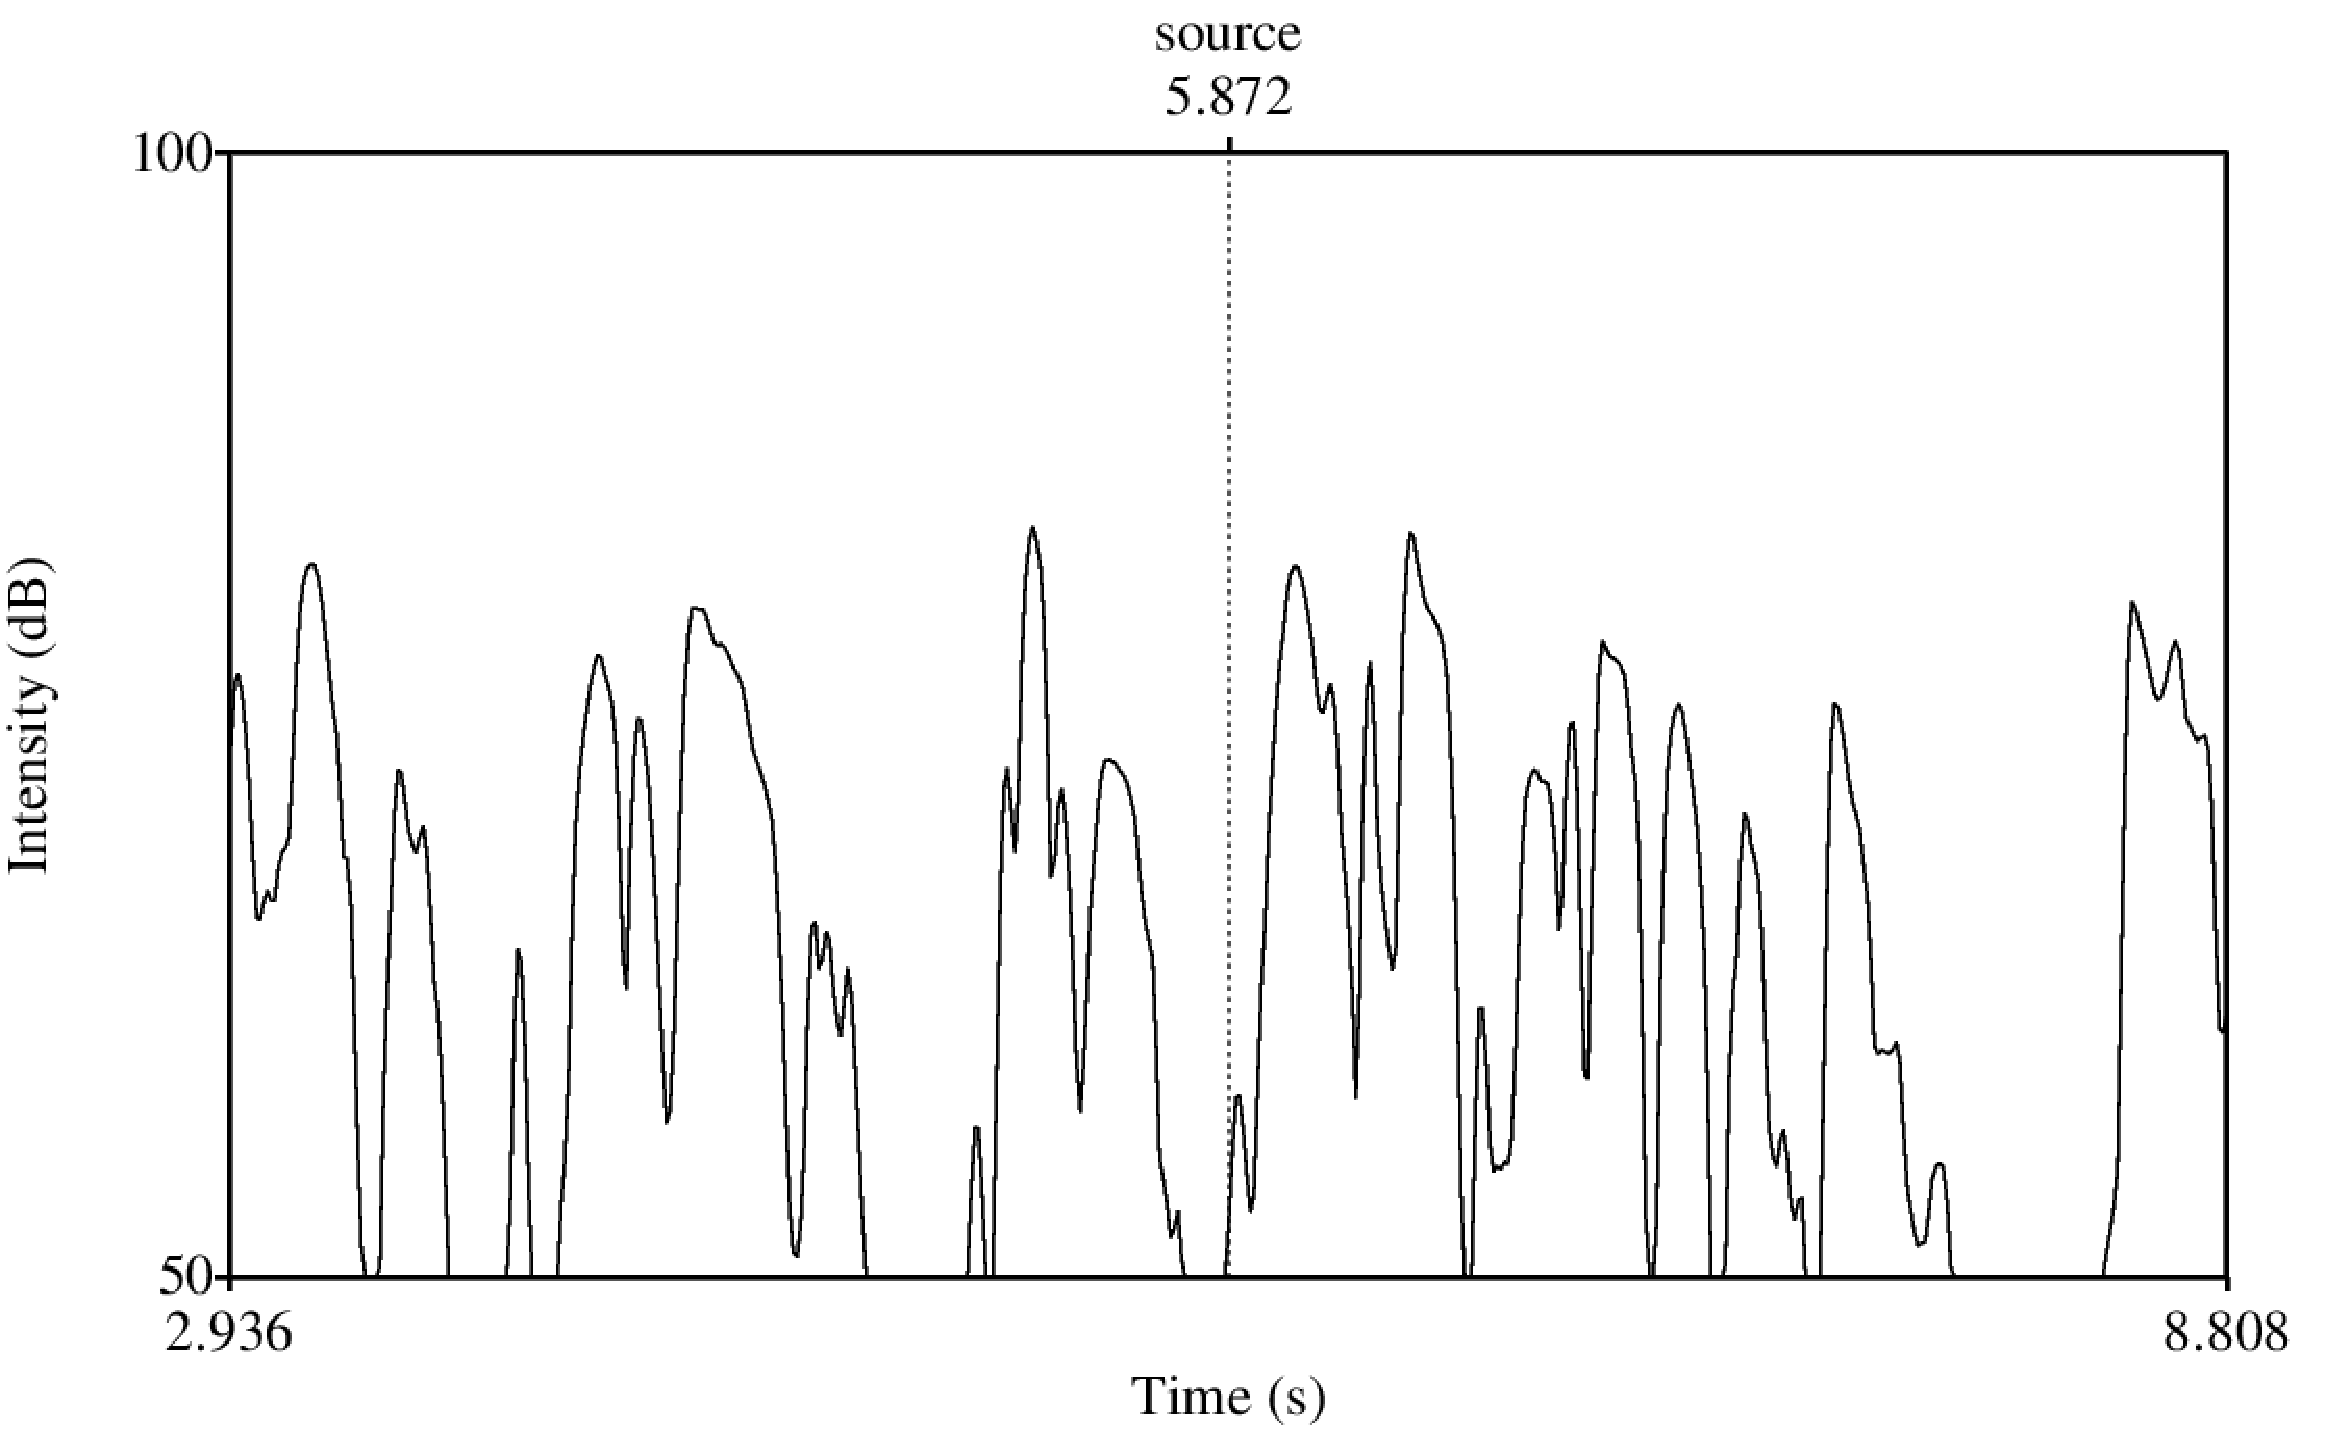
\includegraphics[width=4.5cm, height=3cm]{intorig-eps-converted-to.pdf}%
%\label{fig:intorig}
}
\hfil
\subfigure[Decoder 1 output file]{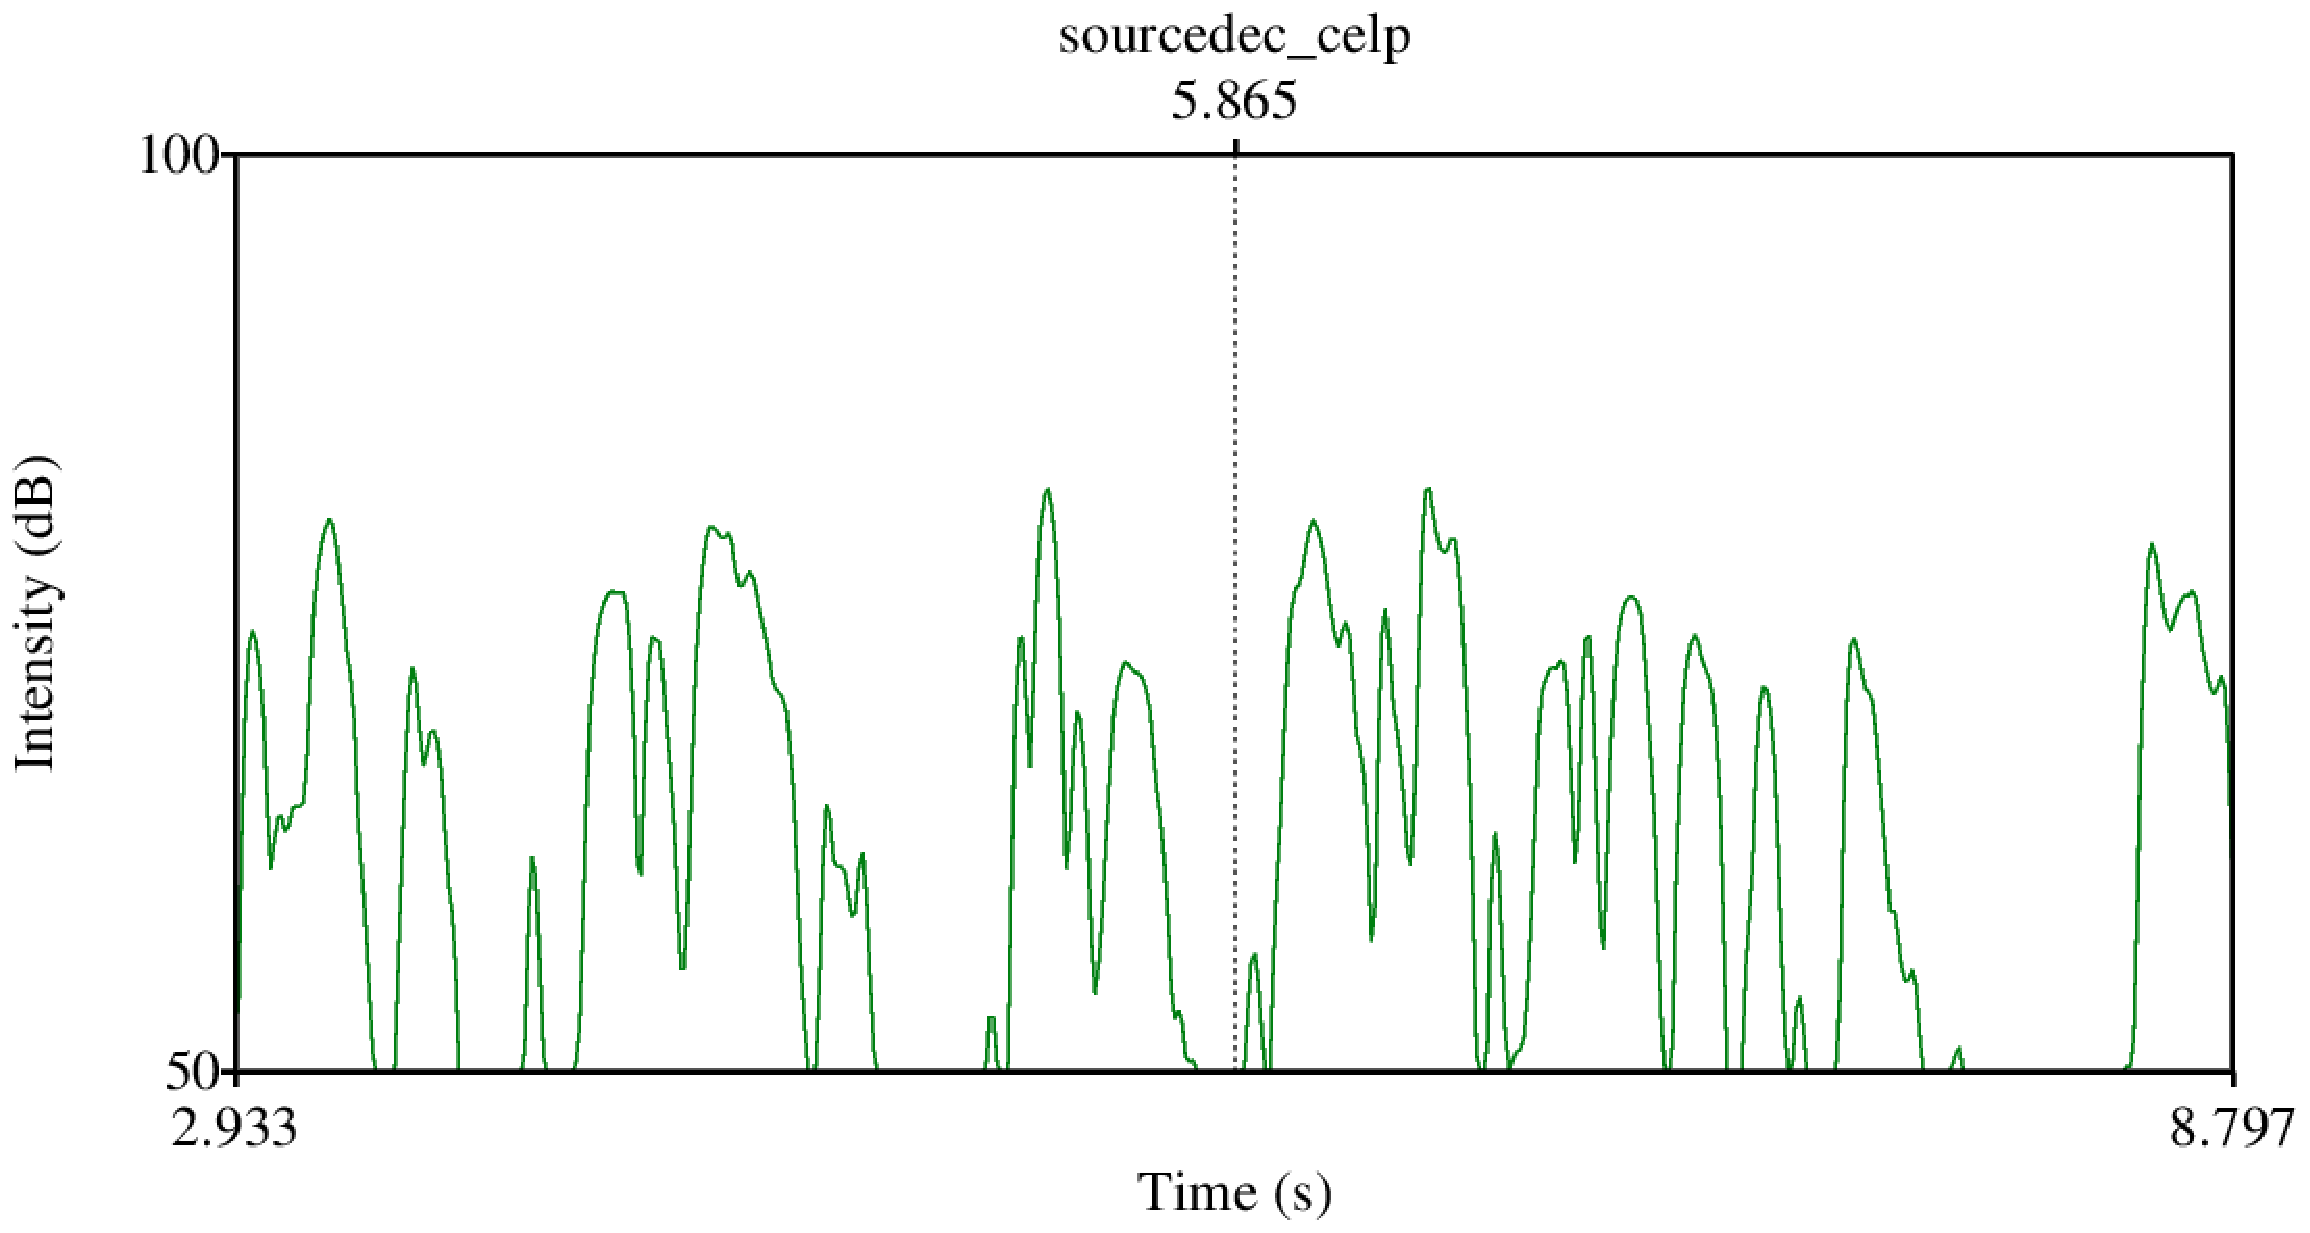
\includegraphics[width=4.5cm, height=3cm]{intcelp-eps-converted-to.pdf}%
%\label{fig:intcelp}
}}
\centerline{\subfigure[Decoder 2 output File]{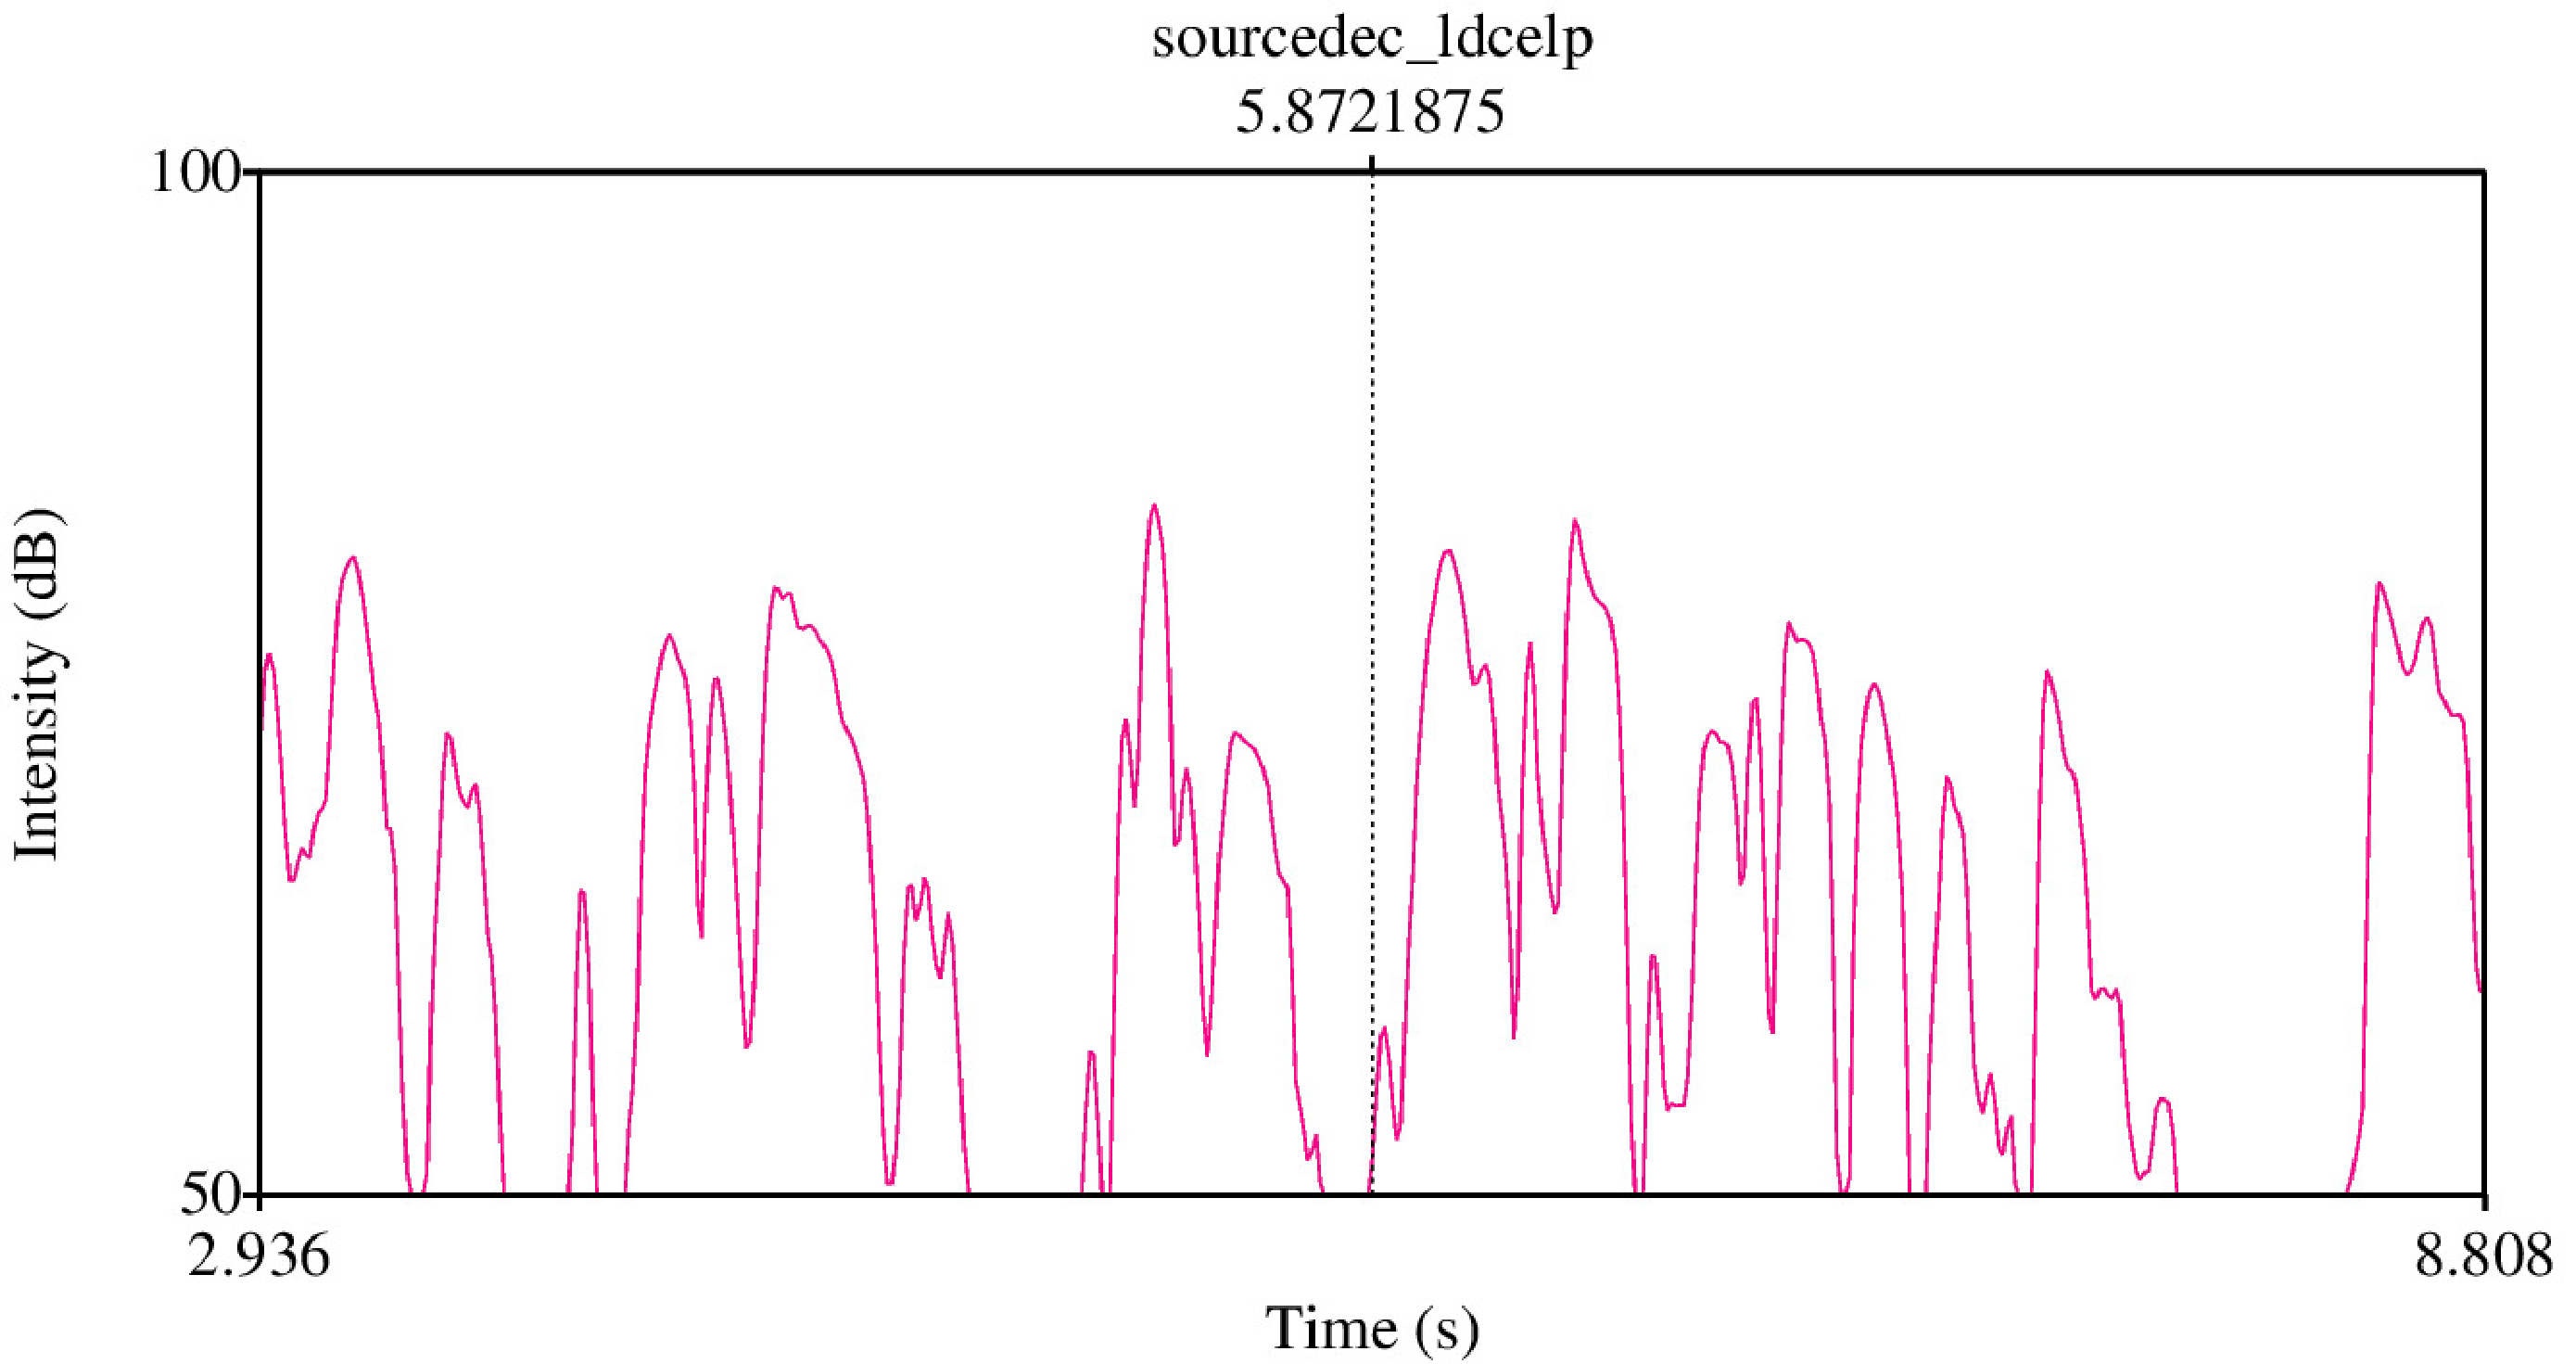
\includegraphics[width=4.5cm, height=3cm]{intldcelp-eps-converted-to.pdf}%
%\label{fig:intldcelp}
}
\hfil
\subfigure[Decoder 3 output file]{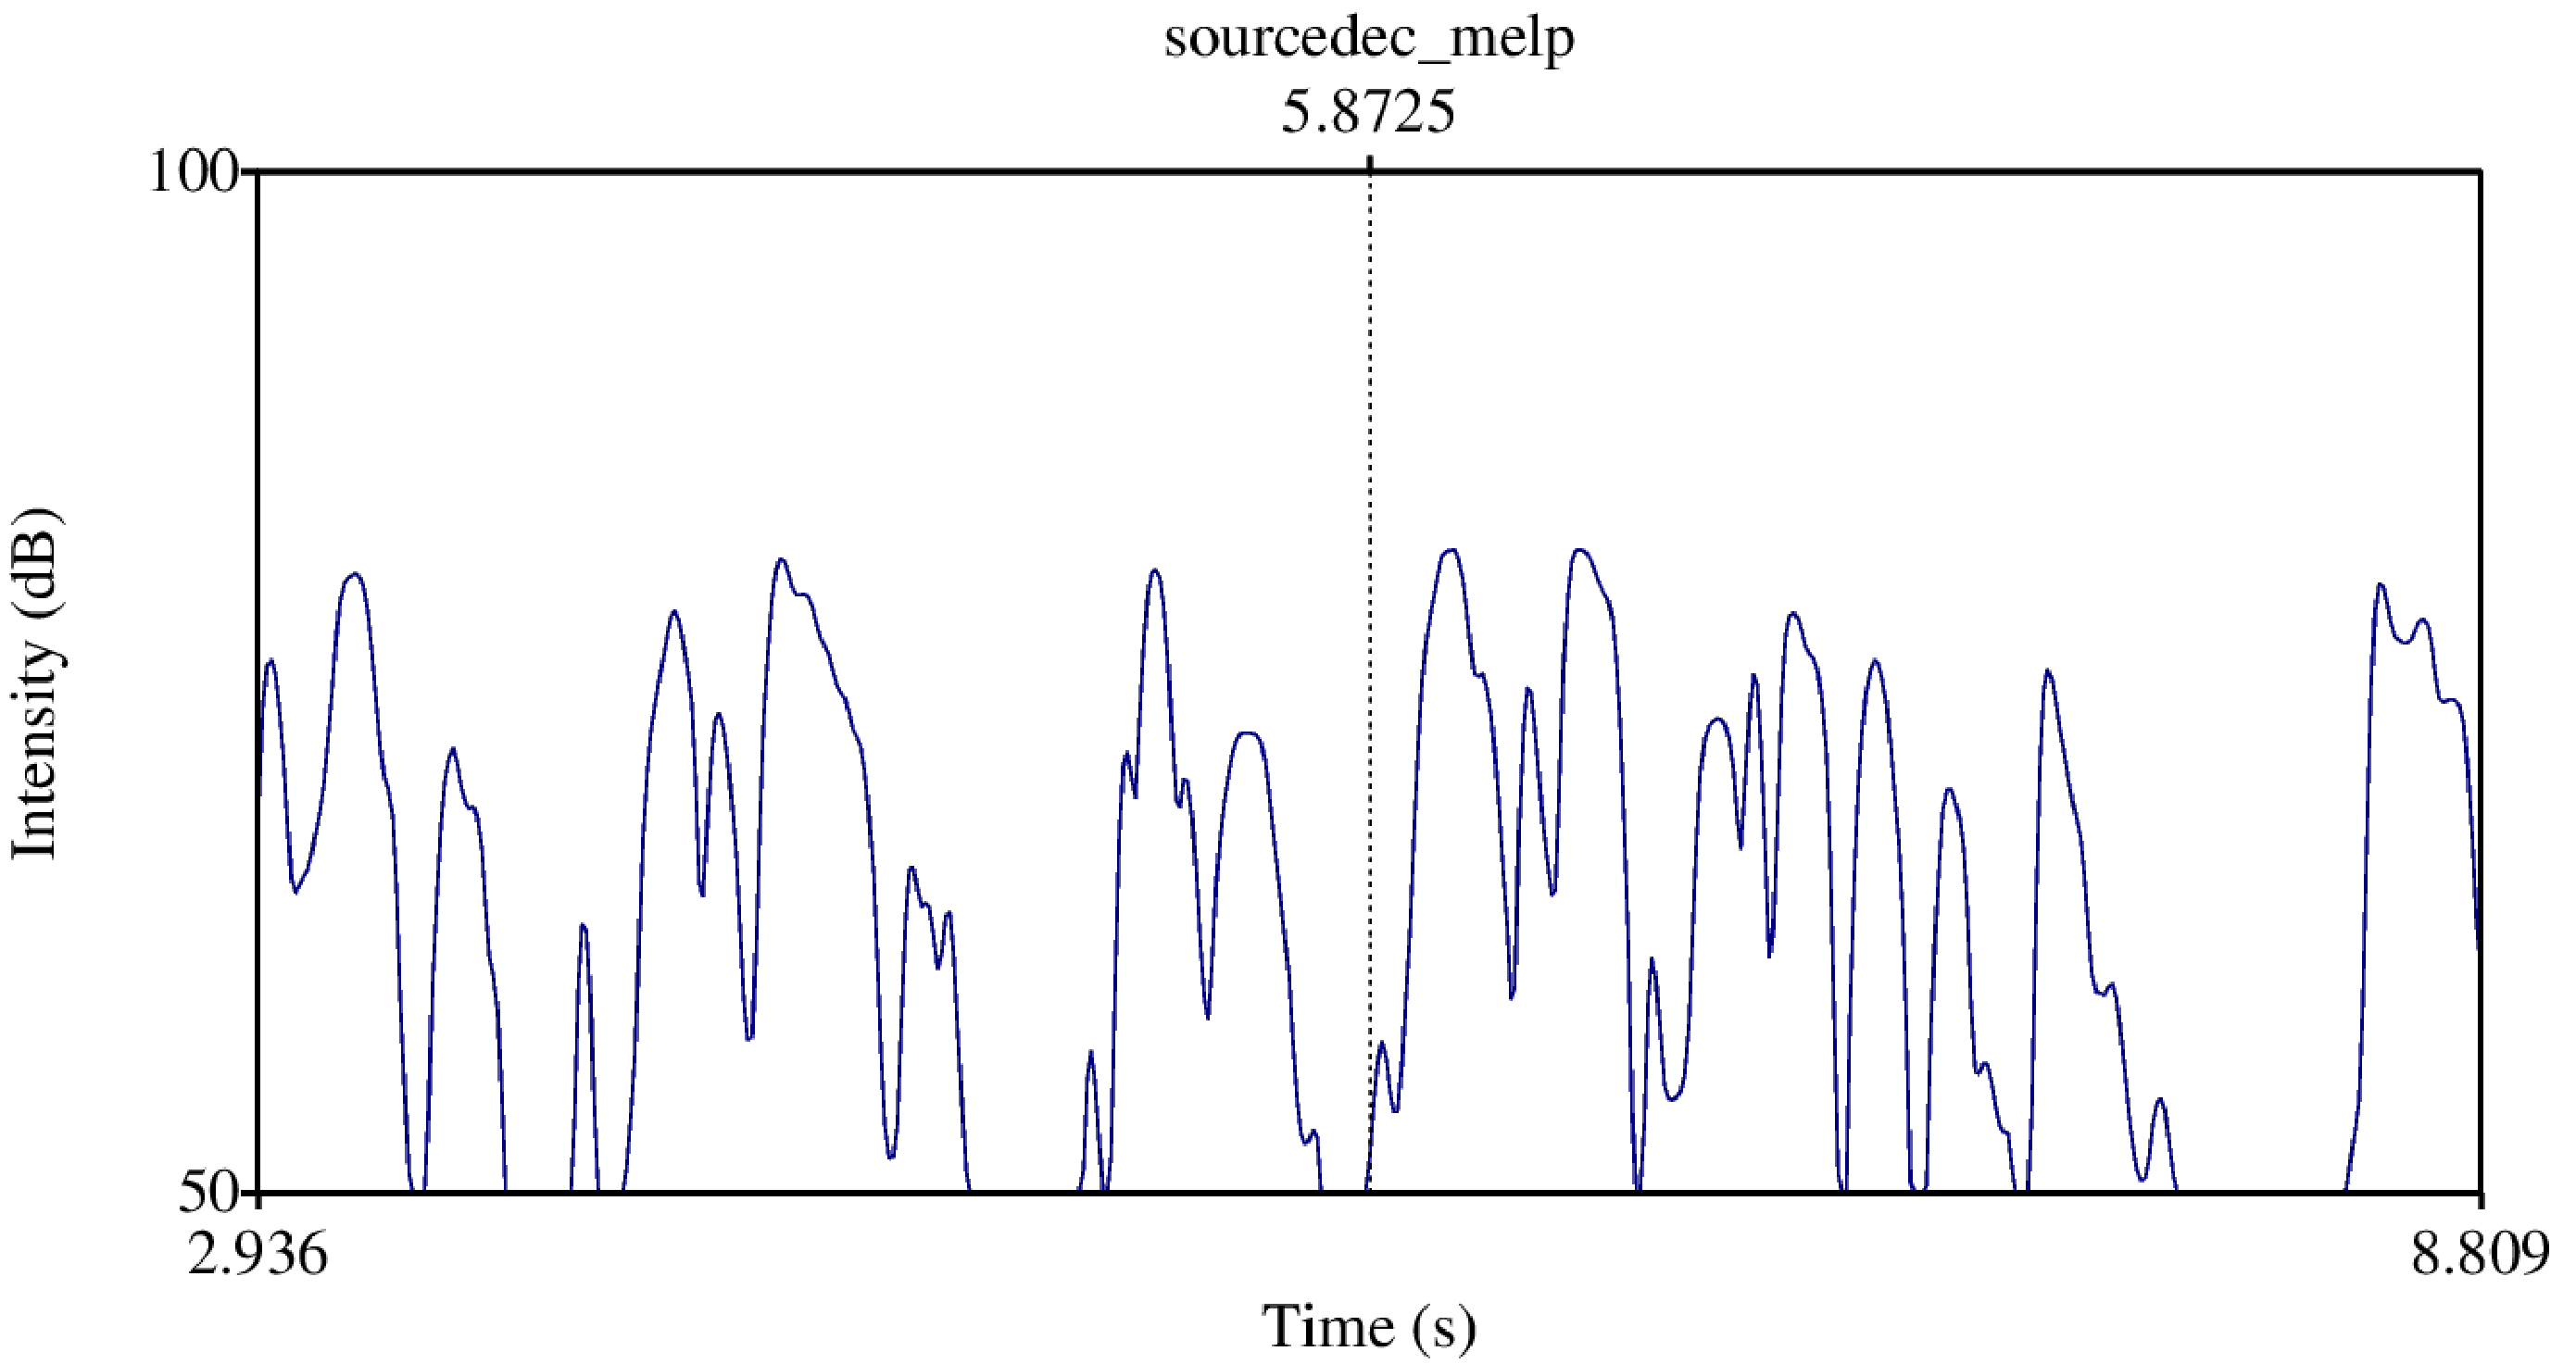
\includegraphics[width=4.5cm, height=3cm]{intmelp-eps-converted-to.pdf}%
%\label{fig:intmelp}
}
}
\caption{An Example showing Sub-figures}
\label{fig:int}
\end{figure*}


\subsubsection{Examples of tables}
\indent Tables may be formatted as in Table~\ref{tab:Table}.
\begin{table}[h]
	\renewcommand{\arraystretch}{1.1}
	\caption{An Example Table}
	\label{tab:Table}
	\centering
	\begin{tabular}{|c|c|c|c|}
		\hline
		Parameter 		& Algorithm 1 	&  	Algorithm 2 	& 	Algorithm 3	\\
		\hline

		file1.wav 		& 3.27		&	3.93		&	2.73 		\\
		file2.wav 		& 3.53		&	4.07		&	2		\\
		file3.wav 		& 3.53		&	4.47		&	2.8 		\\ \hline

		\hline 
		\textbf{Average Value}	& \textbf{3.44} &  \textbf{4.16} & \textbf{2.51}\\ \hline
	\end{tabular}
\end{table}


\indent If vertical lines are not required, tables may be formatted as in Table~\ref{tab:Table_novert}.
\begin{table}[h]
	\renewcommand{\arraystretch}{1.1}
	\caption{An Example Table}
	\label{tab:Table_novert}
	\centering
	\begin{tabular}{cccc}
		\hline
		Parameter 		& Algorithm 1 	&  	Algorithm 2 	& 	Algorithm 3	\\
		\hline

		file1.wav 		& 3.27		&	3.93		&	2.73 		\\
		file2.wav 		& 3.53		&	4.07		&	2		\\
		file3.wav 		& 3.53		&	4.47		&	2.8 		\\ \hline

		\hline 
		\textbf{Average Value}	& \textbf{3.44} &  \textbf{4.16} & \textbf{2.51}\\ \hline
	\end{tabular}
\end{table}


